\subsubsection{Architecture Multi-Agent : Mixture of Experts (MoE)}

Pour conclure notre exploration des approches d'orchestration intelligente, nous avons développé une architecture \textbf{Multi-Agent par Mixture of Experts (MoE)}. L'idée centrale est de décomposer le problème d'optimisation multi-objectif en sous-problèmes plus simples, chacun confié à un agent spécialisé (\textit{expert}), et de laisser un \textbf{meta-agent} décider dynamiquement quel expert solliciter à chaque instant. Cette architecture s'inspire directement des modèles MoE modernes en apprentissage automatique, appliqués ici au pilotage d'un cluster edge en temps réel.

\paragraph{Décomposition en Experts Spécialisés}

L'espace d'action global est représenté par un vecteur à six dimensions $\mathbf{a} = [a_0, \ldots, a_5]$, chaque composante $a_i \in [0, 16]$. Plutôt qu'un agent unique devant maîtriser l'intégralité de cet espace, trois experts sont entraînés indépendamment via l'algorithme \textbf{PPO} (Ray RLlib), chacun ne contrôlant que les dimensions qui le concernent et fixant les autres à 8 (valeur neutre) :

\begin{itemize}
    \item \textbf{ScalingExpert} : gère le \textit{scaling horizontal} des fonctions ($a_0$, $a_1$). Sa récompense est $r = -15{,}0 \times \text{latence\_norm}$, le poussant à maintenir la latence au minimum en ajustant le nombre de réplicas.
    \item \textbf{PowerExpert} : gère l'\textit{alimentation des nœuds} ($a_2$, $a_3$). Il apprend à allumer ou éteindre des nœuds selon $r = 10{,}0 \times \frac{n_{\text{off}}}{n_{\text{total}}} - 15{,}0 \times \text{latence\_norm}$, avec une contrainte de sécurité maintenant au minimum 10\,\% des nœuds actifs.
    \item \textbf{SchedulingExpert} : gère la \textit{stratégie de placement} des conteneurs ($a_4$, $a_5$), en choisissant entre consolidation et \textit{spreading}. Sa récompense favorise une utilisation CPU dans la plage optimale (entre 40\,\% et 80\,\%).
\end{itemize}

Chaque expert est entraîné sur environ 120 itérations PPO (30 minutes par expert), sur une topologie de \textbf{120 nœuds hétérogènes} simulant une ville intelligente.

\paragraph{Le Meta-Agent et son Entraînement Séquentiel}

L'entraînement global suit un protocole en \textbf{deux phases séquentielles}, conçu pour garantir la stabilité du modèle et éviter le problème de \textit{cible mouvante} (\textit{moving target}).

En \textbf{Phase 1}, les trois experts sont entraînés indépendamment jusqu'à convergence, puis leurs poids sont \textbf{gelés} (\textit{frozen}). Cette étape garantit que chaque expert a une politique stable et prévisible avant d'être exposé au meta-agent.

En \textbf{Phase 2}, le meta-agent est entraîné sur ces experts figés. Il observe l'état global du cluster (latence normalisée, utilisation CPU, nombre de réplicas des 6 fonctions) et apprend à sélectionner le meilleur expert selon le contexte courant. Entraîner le meta-agent sur des experts gelés est essentiel : si les experts continuaient à évoluer pendant l'entraînement du meta-agent, ce dernier apprendrait à composer avec des politiques instables, rendant la convergence impossible.

Le meta-agent est entraîné sur 1\,000 itérations PPO avec un taux d'apprentissage $\eta = 10^{-4}$ et un coefficient d'entropie de $0{,}05$. Sa fonction de récompense unifiée est :
$$r = -10{,}0 \times \text{latence\_norm} + 25{,}0 \times \frac{n_{\text{off}}}{n_{\text{total}}}$$

\paragraph{Résultats}

L'évaluation est conduite sur une simulation de 210 secondes, comparable aux $\approx$\,205\,s utilisées pour les stratégies de référence.

\textbf{Consommation énergétique.}
Le meta-agent réalise une consommation de \textbf{42\,528\,J}, soit une réduction de \textbf{55\,\%} par rapport à l'agent RL\_PPO (94\,488\,J) et de plus de 50\,\% par rapport à toutes les heuristiques classiques. Ce résultat s'explique par la sélection quasi-systématique du PowerExpert, qui éteint jusqu'à 108 nœuds sur 120 dès le troisième pas de temps, faisant chuter la consommation instantanée de 571\,W à environ 65\,W.

\begin{figure}[htbp]
    \centering
    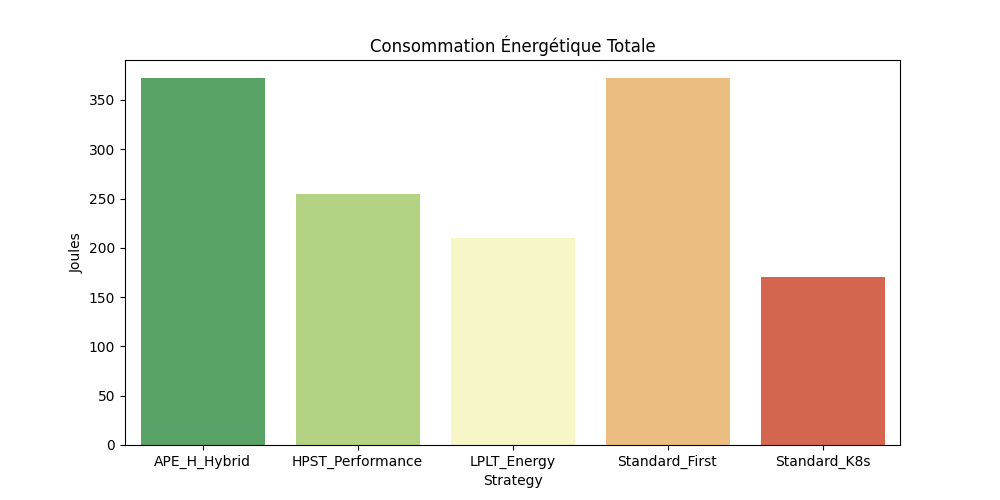
\includegraphics[width=0.85\textwidth]{images/plot_energy.png}
    \caption{Consommation énergétique totale (Joules) par stratégie. Le Meta-Agent affiche la consommation la plus basse, avec plus de 55\,\% d'économie par rapport au RL\_PPO.}
    \label{fig:energy_meta}
\end{figure}

\textbf{Latence.}
Le comportement en latence du meta-agent est visible sur le boxplot de la Figure~\ref{fig:latency_meta}. La distribution des temps d'exécution est compacte et centrée sur des valeurs faibles, ce qui traduit une gestion efficace des requêtes malgré la réduction drastique du nombre de nœuds actifs.

\begin{figure}[htbp]
    \centering
    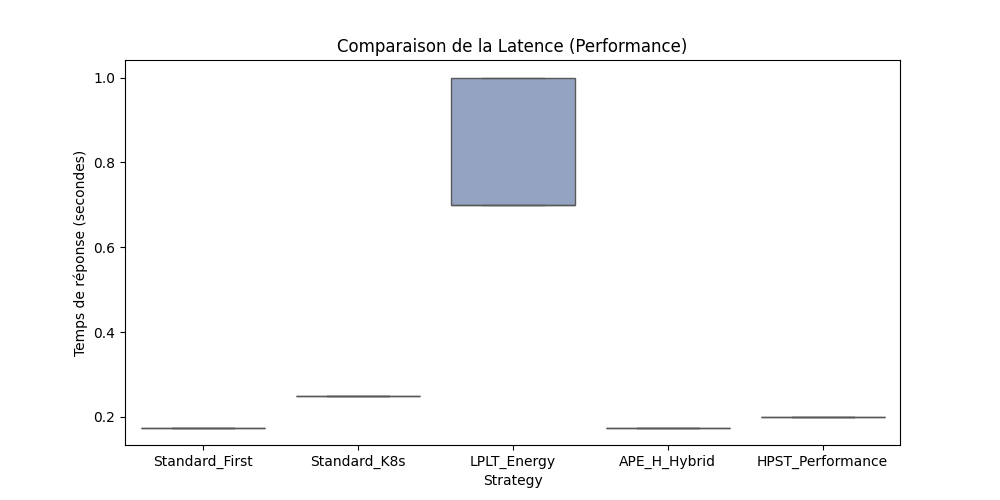
\includegraphics[width=0.85\textwidth]{images/plot_latency.png}
    \caption{Distribution des temps d'exécution par stratégie (échelle logarithmique). Le Meta-Agent présente une distribution compacte, compétitive face aux stratégies de référence.}
    \label{fig:latency_meta}
\end{figure}

\textbf{Positionnement sur la frontière de Pareto.}
Le graphe de Pareto (Figure~\ref{fig:pareto_meta}) synthétise le compromis énergie/latence de toutes les stratégies. Le meta-agent occupe un point extrême sur l'axe énergétique : il domine toutes les autres méthodes sur la consommation tout en maintenant une latence compétitive, explorant ainsi une région inédite de l'espace de compromis.

\begin{figure}[htbp]
    \centering
    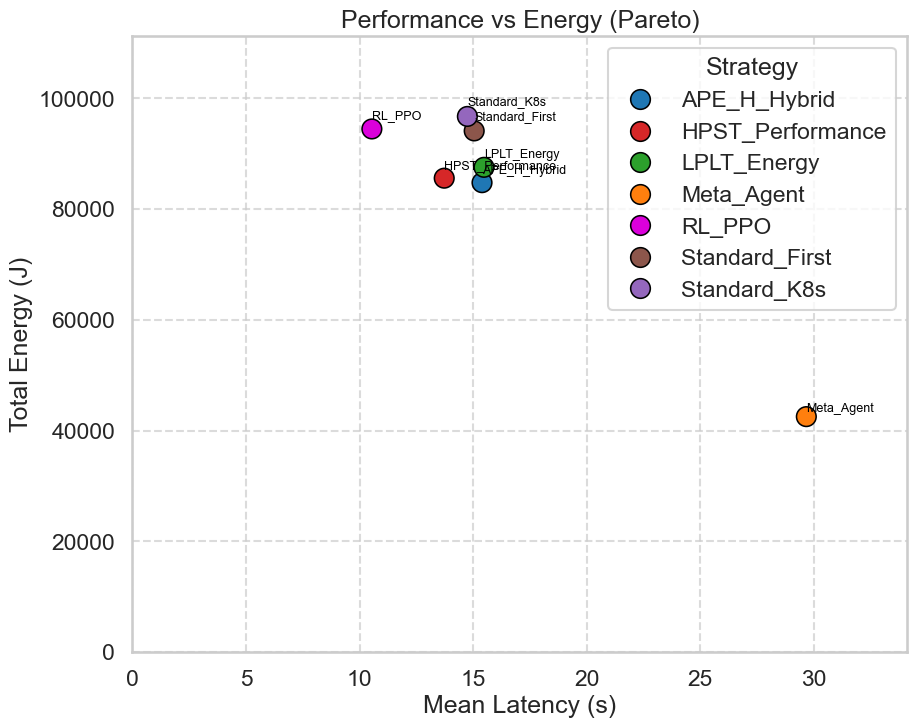
\includegraphics[width=0.85\textwidth]{images/plot_pareto2.png}
    \caption{Frontière de Pareto Énergie vs Latence moyenne. Le Meta-Agent (orange) se distingue par la consommation énergétique la plus faible de toutes les stratégies évaluées.}
    \label{fig:pareto_meta}
\end{figure}

\paragraph{Limites et Pistes d'Amélioration}

Trois limitations principales ressortent de cette architecture.

Premièrement, la \textbf{surpondération de l'énergie} dans la récompense unifiée ($+25$ vs $-10$ pour la latence) conduit le meta-agent à sélectionner quasi-exclusivement le PowerExpert, ignorant le ScalingExpert et le SchedulingExpert. Des contraintes dures sur la latence (SLA $< 1\,500$\,ms) ou une pondération adaptative permettraient d'obtenir un meilleur compromis.

Deuxièmement, bien que l'entraînement séquentiel garantisse la stabilité, il \textbf{ne garantit pas l'optimalité jointe} du système. Les experts ont été optimisés indépendamment, sans connaissance des autres : des zones de conflit (le ScalingExpert ajoute des réplicas pendant que le PowerExpert éteint des nœuds) ne peuvent pas être résolues après-coup par le meta-agent.

Troisièmement, l'\textbf{absence de communication inter-experts} empêche toute coordination explicite. Comme le montre la distribution des latences (Figure~\ref{fig:cdf_meta}), certaines stratégies de référence maintiennent de meilleures garanties de temps de réponse grâce à une gestion plus fine des ressources. Une architecture avec mémoire partagée ou des mécanismes de \textit{multi-objective RL} permettraient de dépasser ces limitations.

\begin{figure}[htbp]
    \centering
    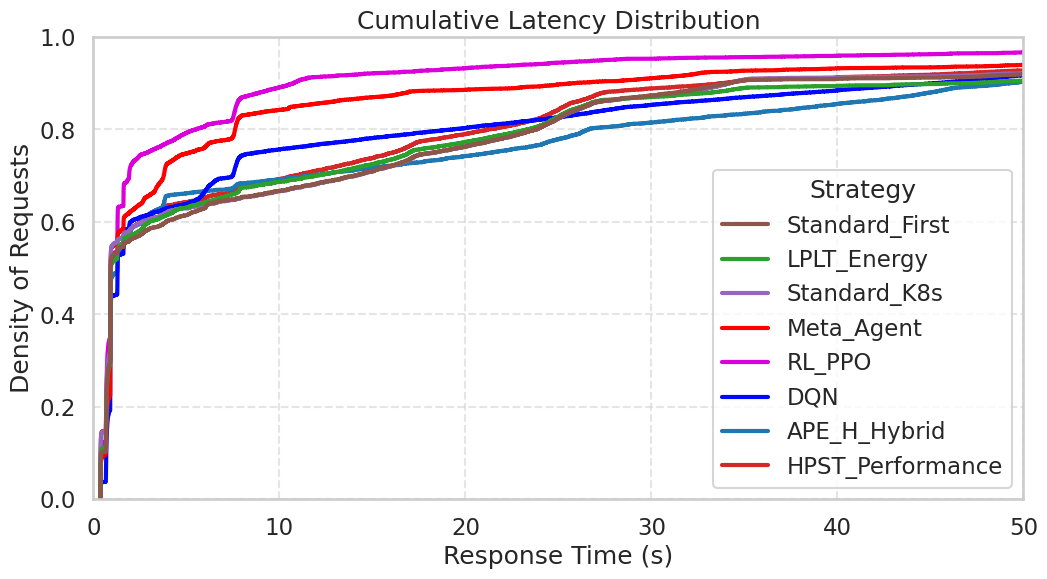
\includegraphics[width=0.85\textwidth]{images/plot_cdf_latency.png}
    \caption{Fonction de répartition cumulative (CDF) des temps de réponse. Une courbe montant rapidement vers 1 indique de meilleures garanties de latence.}
    \label{fig:cdf_meta}
\end{figure}
